% !TeX document-id = {3c518733-43c3-4789-8e54-51d5112a1304}
% !TeX program = lualatex
% !BIB program = biber
% Lualatex is important to render TTF fonts; with pdflatex it's just the regular one
% ratio 16:9 -- https://tex.stackexchange.com/questions/14336/

% compile two versions, inspired by https://tex.stackexchange.com/a/1501
% use the script "compile-pdf.sh"
\newif\ifhandout
% if flags.tex does not exist, create an empty file to be able to compile in TeXstudio
\input{flags}

\ifhandout
	\documentclass[12pt,aspectratio=169,handout]{beamer}
\else
	\documentclass[12pt,aspectratio=169]{beamer}
\fi

% adjust for 16:9
% https://tex.stackexchange.com/questions/354022/modifying-the-margins-of-all-slides-in-beamer
\setbeamersize{text margin left=0.3cm,text margin right=4.5cm} 

%\usepackage{xcolor}

% use Metropolis as the basis theme
\usetheme[subsectionpage=progressbar]{metropolis}
% blocks with background globally
\metroset{block=fill}

% ------- Paderborn specifics ----------
\usepackage{fontspec}
%\setsansfont{karla} % looked bad, too fat
\setsansfont{Segoe UI} % looks OK-ish

% Paderborn color scheme
\definecolor{UPBUltraBlue}{RGB}{0, 37, 170}

\setbeamercolor{frametitle}{bg=white, fg=UPBUltraBlue}

% name in footer
\setbeamertemplate{frame numbering}{Prof.\ Dr.\ Ivan Habernal ~ | ~ \insertframenumber }

% adjust the background to be completely white
\setbeamercolor{background canvas}{bg=white}

% add Paderborn logo at each slide
% actually not -- it's just eating up space
%\addtobeamertemplate{frametitle}{}{%
%\begin{tikzpicture}[remember picture,overlay]
%	\node[anchor=north east,yshift=2pt] at (current page.north east) {
\includegraphics[height=0.9cm]{img/UPB_Logo_ENG_coloured_RGB}};
%\end{tikzpicture}
%}

% show TOC at every section start
\AtBeginSection{
	\frame{
		\vspace{2em}
		\sectionpage
		\hspace*{2.2em}\begin{minipage}{10cm}
			\tableofcontents[currentsection]
		\end{minipage}
		% we need the logo to show up here as well
		\begin{tikzpicture}[remember picture,overlay]
			\node[anchor=north east,yshift=2pt] at (current page.north east) {
\includegraphics[height=0.9cm]{img/UPB_Logo_ENG_coloured_RGB}};
		\end{tikzpicture}
	}
}
% ------- end of Paderborn specifics ----------


% typeset mathematics on serif
\usefonttheme[onlymath]{serif}

% better bibliography using biber as backend
\usepackage[natbib=true,backend=biber,style=authoryear-icomp,maxbibnames=30,maxcitenames=9,uniquelist=false,giveninits=true,doi=false,url=false,dashed=false,isbn=false]{biblatex}
% shared bibliography
\addbibresource{../nlpwdl-bibliography.bib}
% disable "ibid" for repeated citations
\boolfalse{citetracker}



\usepackage{xspace}


% for derivatives, https://tex.stackexchange.com/a/412442
\usepackage{physics}

\usepackage{tikz}
\usetikzlibrary{matrix, positioning}
\usetikzlibrary{angles,quotes} % for angles
\usetikzlibrary{backgrounds} % background
\usetikzlibrary{decorations.pathreplacing} % curly braces
\usetikzlibrary{calligraphy}
\usetikzlibrary{calc} % for neural nets

% for plotting functions
\usepackage{pgfplots}
\usepgfplotslibrary{dateplot}

% sub-figures
\usepackage{caption}
\usepackage{subcaption}

% book tabs
\usepackage{booktabs}


% argmin, argmax
\usepackage{amsmath}
\DeclareMathOperator*{\argmax}{arg\!\max}
\DeclareMathOperator*{\argmin}{arg\!\min}
% softmax
\DeclareMathOperator*{\softmax}{soft\!\max}

% bold math
\usepackage{bm}

% for \mathclap
\usepackage{mathtools}

% algorithms
\usepackage[noend]{algpseudocode}


% for neurons and layers in tikz
\tikzset{
	neuron/.style={draw, rectangle, inner sep=2pt, minimum width=0.75cm, fill=blue!20},
	param/.style={draw, rectangle, inner sep=2pt, minimum width=0.75cm, fill=green!20},
	constant/.style={draw, rectangle, inner sep=2pt, minimum width=0.75cm, fill=black!15},
	% for citation nodes right top
	ref/.style={anchor = north east, text width=7.8cm, yshift=-1.3cm, xshift=-0.2cm, scale=0.5}
}

\title{Natural Language Processing with Deep Learning}
\subtitle{Lecture 5 --- Text generation 1: Language models and word embeddings}
\date{November 10, 2023}
\author{Prof.\ Dr.\ Ivan Habernal}
\institute{Natural Language Processing Group 
\hfill 
\includegraphics[height=1.4cm]{img/UPB_Logo_ENG_coloured_RGB} \\
Paderborn University \\
We focus on Trustworthy Human Language Technologies \hfill \texttt{www.trusthlt.org} }


\begin{document}

\maketitle



\section{Finishing previous lecture: Stacking layers, non-linearity}


\begin{frame}
	\begin{figure}
		\vspace{-1.3em}
		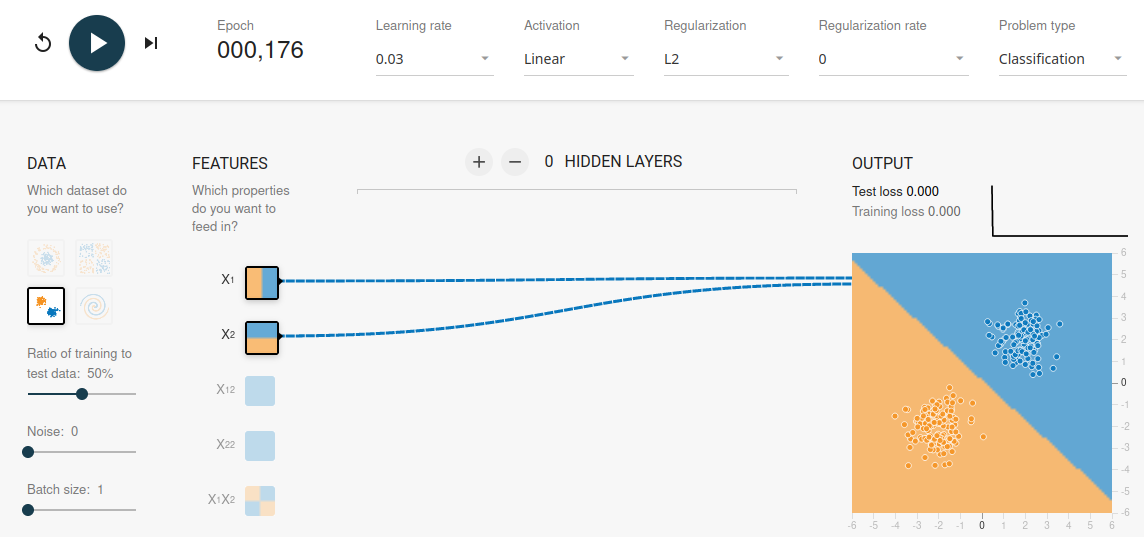
\includegraphics[width=1.35\linewidth]{img/linear1.png}	
		\caption{Linear model can tackle only linearly-separable problems (\url{http://playground.tensorflow.org})}
	\end{figure}	
\end{frame}

\begin{frame}
	\begin{figure}
		\vspace{-1.3em}
		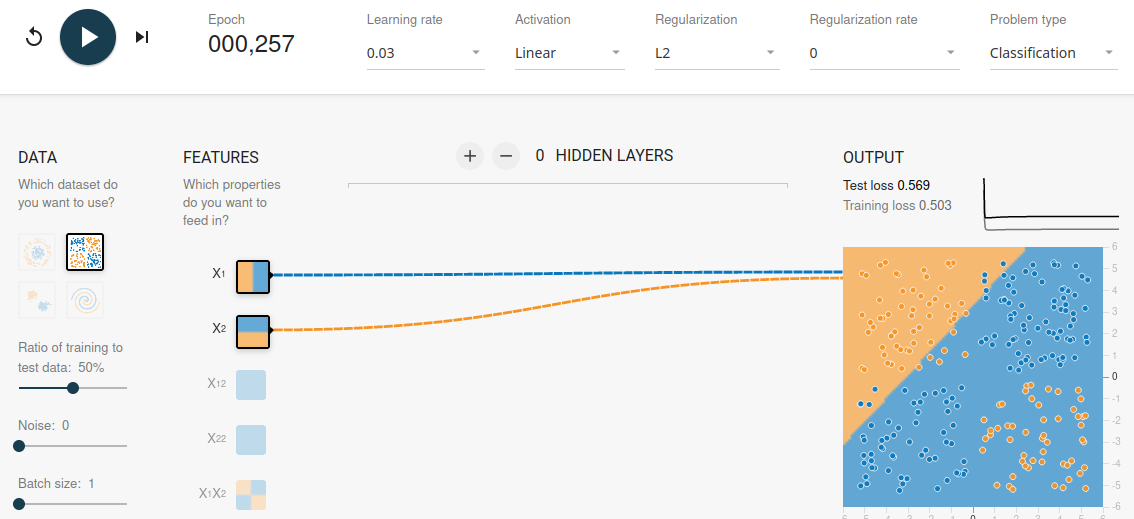
\includegraphics[width=1.35\linewidth]{img/linear2.png}	
		\caption{Linear model can tackle only linearly-separable problems (\url{http://playground.tensorflow.org})}
	\end{figure}	
\end{frame}


\begin{frame}{Stacking linear layers on top of each other --- still linear!}
	\vspace{-1em}
	$$
	\bm{x} \in \mathbb{R}^{d_{in}} \qquad
	\bm{W^1} \in \mathbb{R}^{d_{in} \times d_1} \qquad
	\bm{b^1} \in \mathbb{R}^{d_1} \qquad
	\bm{W^2} \in \mathbb{R}^{d_1 \times d_{out}} \qquad
	\bm{b^2} \in \mathbb{R}^{d_{out}} \qquad
	$$
	$$
	f(\bm{x}) = \left(
	\bm{x} \bm{W^1} + \bm{b^1}
	\right)
	\bm{W^2} + \bm{b^2}
	$$
	
	\begin{figure}
		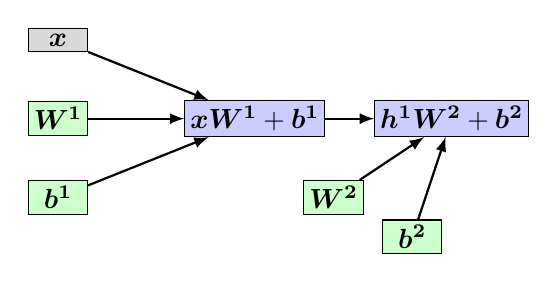
\begin{tikzpicture}	
			%\node (a1) [draw, circle, inner sep=0pt, minimum width=0.75cm, fill=green!20] {$a_1$};
			\node (x) [constant] {$\bm{x}$};
			\node (w) [param, below of=x] {$\bm{W^1}$};
			\node (b) [param, below of=w] {$\bm{b^1}$};
			
			\node (f1) [neuron, right of=w, xshift=1.5cm] {$\bm{x} \bm{W^1} + \bm{b^1}$};
			\node (f2) [neuron, right of=f1, xshift=1.5cm] {$\bm{h^1} \bm{W^2} + \bm{b^2}$};
			
			\node (w2) [param, below of=f2, xshift=-1.5cm, yshift=0cm] {$\bm{W^2}$};
			\node (b2) [param, below of=f2, xshift=-0.5cm, yshift=-0.5cm] {$\bm{b^2}$};
			
%			\node (l) [neuron, right of=f2, xshift=1cm] {$L$};
%			\node (y) [constant, below of=f2, xshift=1.5cm] {$\bm{y}$};
			
			\begin{scope}[thick, black, ->, >=latex]
				\draw (x) -- (f1);
				\draw (w) -- (f1);
				\draw (b) -- (f1);
				\draw (f1) -- (f2);
%				\draw (f2) -- (l);
				\draw (w2) -- (f2);
				\draw (b2) -- (f2);
%				\draw (y) -- (l);
			\end{scope}	
		\end{tikzpicture}
		\caption{Computational graph; green boxes are trainable parameters, gray are constant inputs}
	\end{figure}	
	
\end{frame}


\begin{frame}
	\begin{figure}
		\vspace{-1.3em}
		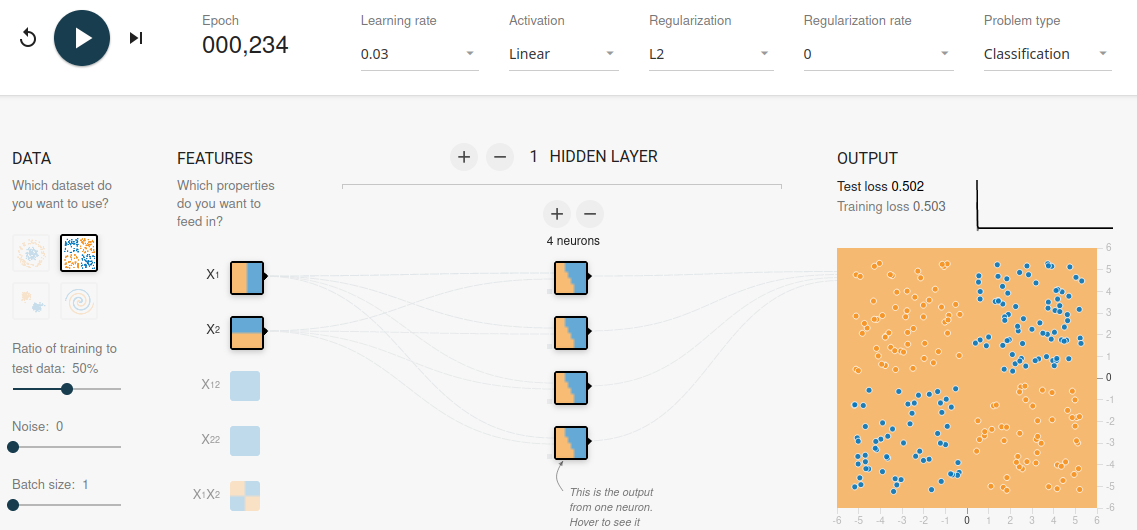
\includegraphics[width=1.35\linewidth]{img/linear3.png}	
		\caption{Linear hidden layers do not help (\url{http://playground.tensorflow.org})}
	\end{figure}	
\end{frame}




\begin{frame}{Adding non-linear function $g: \mathbb{R}^{d_1} \to \mathbb{R}^{d_1}$}
	\vspace{-1em}
	$$
	f(\bm{x}) = g \left(
	\bm{x} \bm{W^1} + \bm{b^1}
	\right)
	\bm{W^2} + \bm{b^2}
	$$
	
	\begin{figure}
		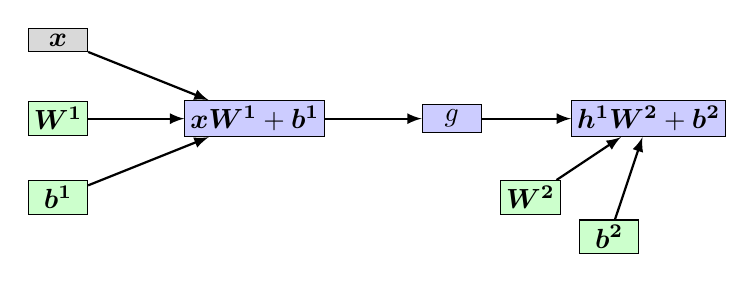
\begin{tikzpicture}	
			%\node (a1) [draw, circle, inner sep=0pt, minimum width=0.75cm, fill=green!20] {$a_1$};
			\node (x) [constant] {$\bm{x}$};
			\node (w) [param, below of=x] {$\bm{W^1}$};
			\node (b) [param, below of=w] {$\bm{b^1}$};
			
			\node (f1) [neuron, right of=w, xshift=1.5cm] {$\bm{x} \bm{W^1} + \bm{b^1}$};
			
			\node (g) [neuron, right of=f1, xshift=1.5cm] {$g$};
			\node (f2) [neuron, right of=g, xshift=1.5cm] {$\bm{h^1} \bm{W^2} + \bm{b^2}$};
			
			\node (w2) [param, below of=f2, xshift=-1.5cm, yshift=0cm] {$\bm{W^2}$};
			\node (b2) [param, below of=f2, xshift=-0.5cm, yshift=-0.5cm] {$\bm{b^2}$};
			
%			\node (l) [neuron, right of=f2, xshift=1cm] {$L$};
%			\node (y) [constant, below of=f2, xshift=1.5cm] {$\bm{y}$};
			
			\begin{scope}[thick, black, ->, >=latex]
				\draw (x) -- (f1);
				\draw (w) -- (f1);
				\draw (b) -- (f1);
				\draw (f1) -- (g);
				\draw (g) -- (f2);
%				\draw (f2) -- (l);
				\draw (w2) -- (f2);
				\draw (b2) -- (f2);
%				\draw (y) -- (l);
			\end{scope}	
		\end{tikzpicture}
		\caption{Computational graph; green boxes are trainable parameters, gray are constant inputs}
	\end{figure}	
	
\end{frame}



\begin{frame}{Non-linear function $g$: Rectified linear unit (ReLU) activation}
	
	
	\begin{columns}
		
		\begin{column}{0.6\linewidth}
			
			$$
			\mathrm{ReLU}(z) =
			\begin{cases}
				0  & \quad \text{if } z < 0\\
				z  & \quad \text{if } z \geq 0
			\end{cases}
			$$
			
			or \hspace{0.4em} $\mathrm{ReLU}(z) = \max(0, x)$
			
			
			
			
		\end{column}
		
		\begin{column}{0.4\linewidth}
			\begin{figure}
				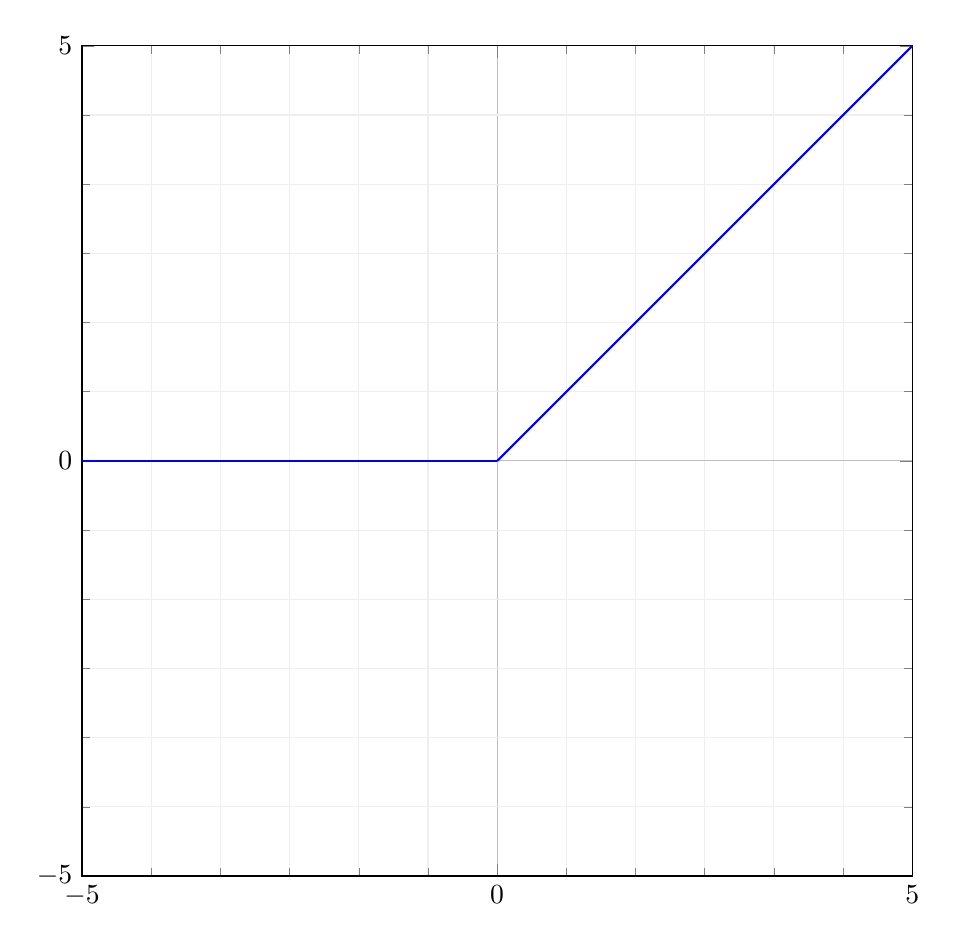
\begin{tikzpicture}
					
					\begin{axis}[
						xmin = -5, xmax = 5,
						ymin = -5, ymax = 5,
						xtick distance = 5,
						ytick distance = 5,
						grid = both,
						minor tick num = 5,
						major grid style = {lightgray},
						minor grid style = {lightgray!25},
						width = \textwidth,
						height = \textwidth,
						legend pos = north west
						]
						
						\addplot[
						domain = -5:0,
						samples = 10,
						smooth,
						thick,
						blue,
						] {0};
						
						\addplot[
						domain = 0:5,
						samples = 10,
						smooth,
						thick,
						blue,
						] {x};
						
						
					\end{axis}
					
				\end{tikzpicture}
				\caption{ReLU function}
			\end{figure}
		\end{column}
	\end{columns}
	
	
\end{frame}


\begin{frame}
	\begin{figure}
		\vspace{-1.3em}
		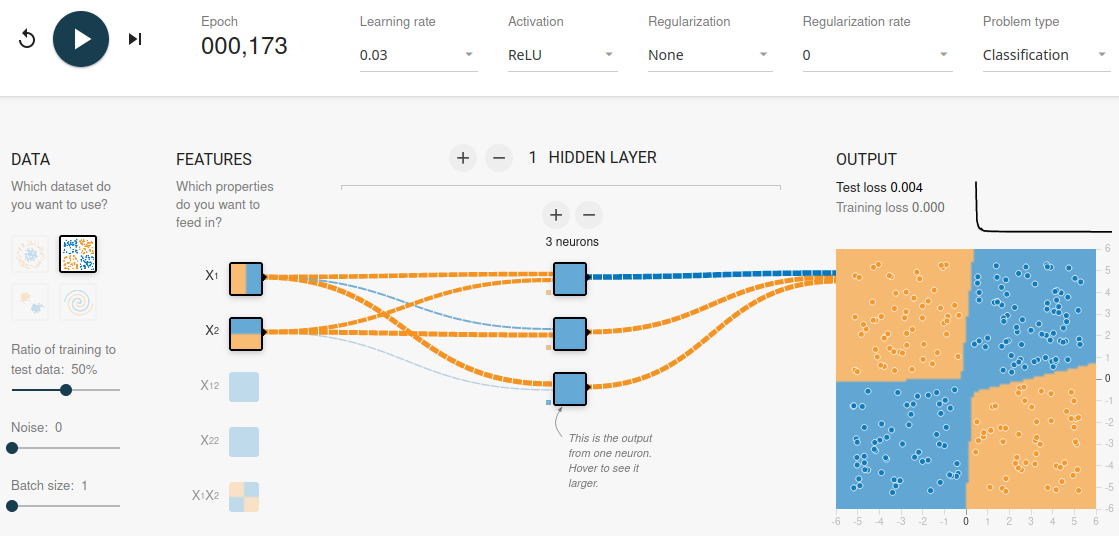
\includegraphics[width=1.35\linewidth]{img/linear4.png}	
		\caption{XOR solvable with, e.g., ReLU (\url{http://playground.tensorflow.org})}
	\end{figure}	
\end{frame}


\begin{frame}{XOR example in super-simplified sentiment classification}
	\begin{figure}
		\vspace{-1.3em}
		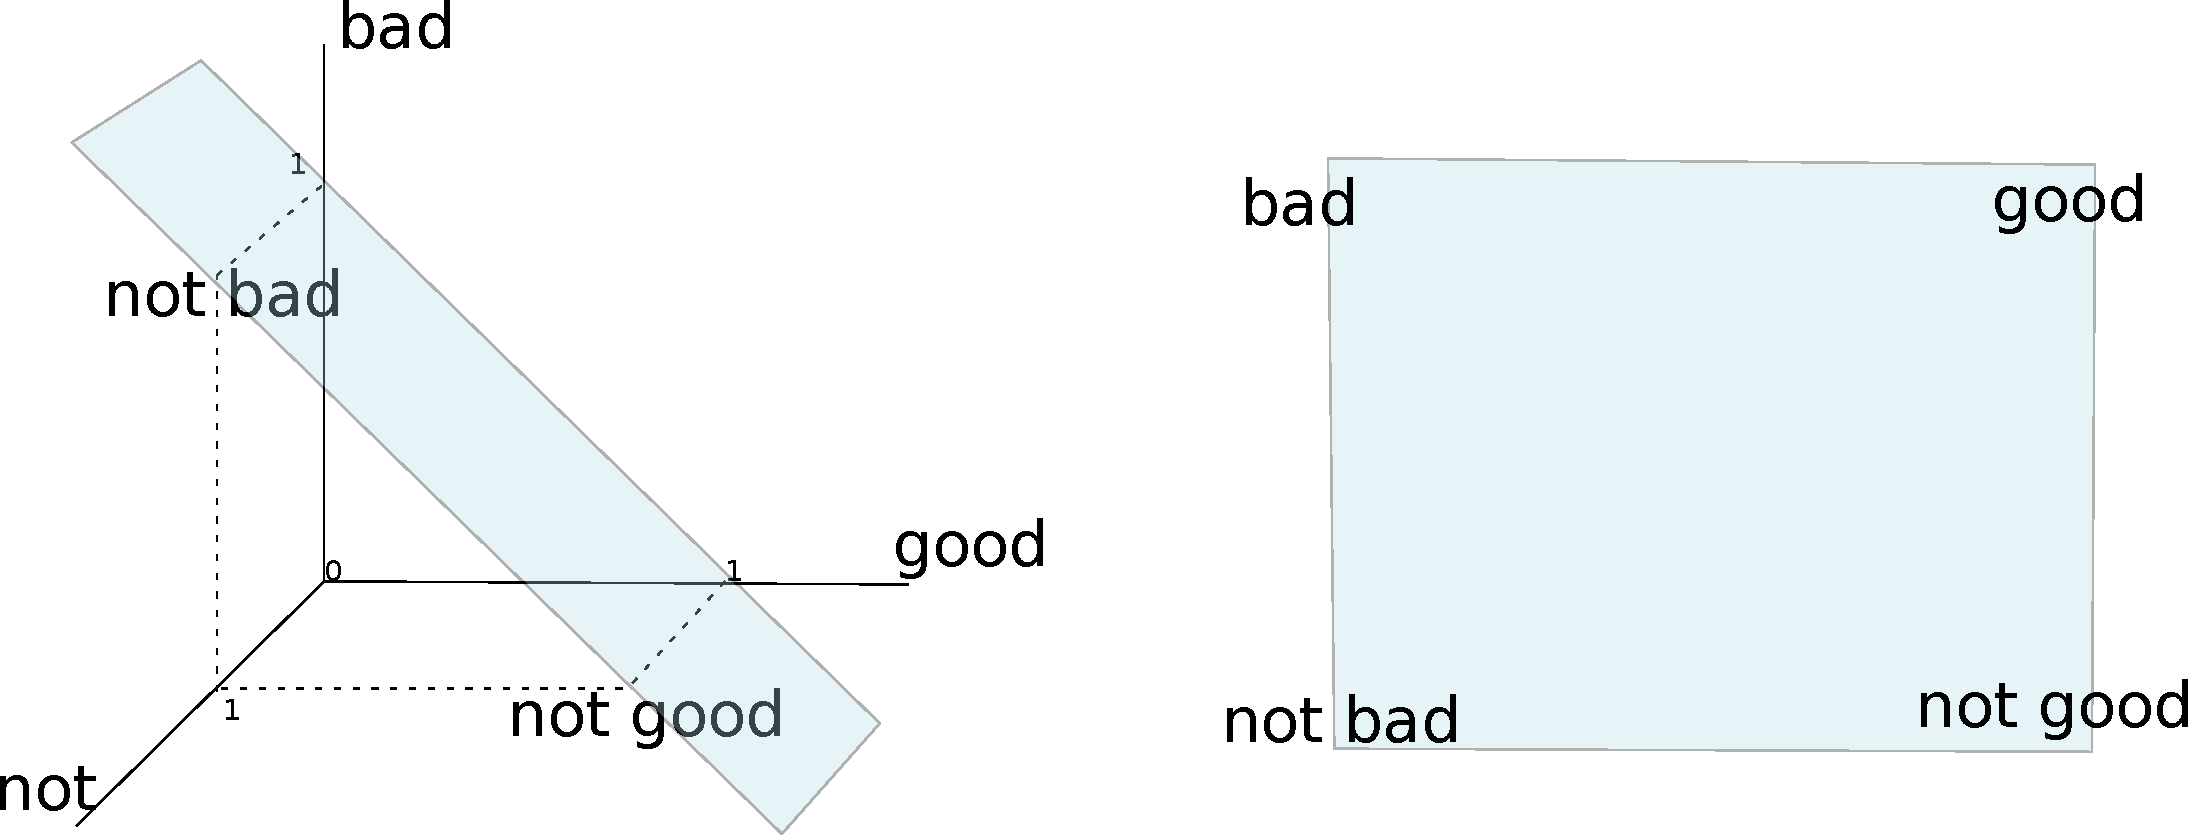
\includegraphics[width=1.2\linewidth]{img/xor1.pdf}	
		\caption{$V = \{\text{not}, \text{bad}, \text{good}\}$, binary features $\in \{0, 1\}$}
	\end{figure}	
\end{frame}




\begin{frame}{Multi-layer perceptron (MLP)}
	\vspace{-1em}
	$$
	f(\bm{x}) = \sigma \left( g \left(
	\bm{x} \bm{W^1} + \bm{b^1}
	\right)
	\bm{W^2} + \bm{b^2} \right)
	$$
	
	\begin{figure}
		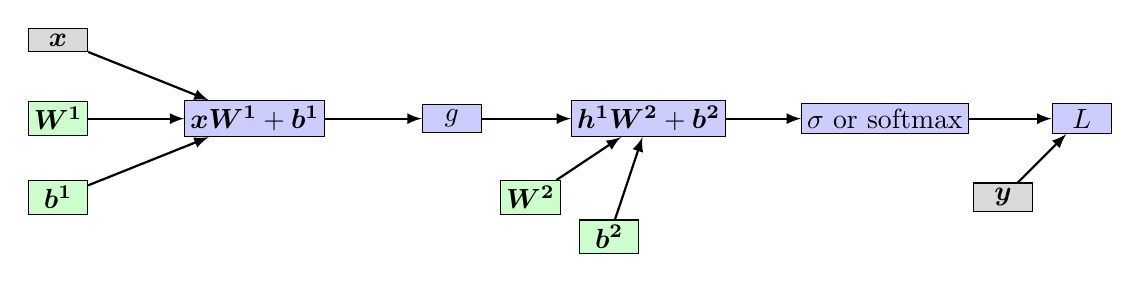
\begin{tikzpicture}	
			%\node (a1) [draw, circle, inner sep=0pt, minimum width=0.75cm, fill=green!20] {$a_1$};
			\node (x) [constant] {$\bm{x}$};
			\node (w) [param, below of=x] {$\bm{W^1}$};
			\node (b) [param, below of=w] {$\bm{b^1}$};
			
			\node (f1) [neuron, right of=w, xshift=1.5cm] {$\bm{x} \bm{W^1} + \bm{b^1}$};
			
			\node (g) [neuron, right of=f1, xshift=1.5cm] {$g$};
			\node (f2) [neuron, right of=g, xshift=1.5cm] {$\bm{h^1} \bm{W^2} + \bm{b^2}$};
			
			\node (w2) [param, below of=f2, xshift=-1.5cm, yshift=0cm] {$\bm{W^2}$};
			\node (b2) [param, below of=f2, xshift=-0.5cm, yshift=-0.5cm] {$\bm{b^2}$};
			
			\node (sigma) [neuron, right of=f2, xshift=2cm] {$\sigma$ or softmax};
			
			\node (l) [neuron, right of=sigma, xshift=1.5cm] {$L$};
			\node (y) [constant, below of=sigma, xshift=1.5cm] {$\bm{y}$};
			
			\begin{scope}[thick, black, ->, >=latex]
				\draw (x) -- (f1);
				\draw (w) -- (f1);
				\draw (b) -- (f1);
				\draw (f1) -- (g);
				\draw (g) -- (f2);
				\draw (f2) -- (sigma);
				\draw (sigma) -- (l);
				\draw (w2) -- (f2);
				\draw (b2) -- (f2);
				\draw (y) -- (l);
			\end{scope}	
		\end{tikzpicture}
		\caption{Computational graph; green boxes are trainable parameters, gray are constant inputs}
	\end{figure}	
	
\end{frame}




\section*{Today: Language models and word embeddings}

\section{Language models}

\subsection{Probability refresher}


\begin{frame}{Probability refresher 1}
	
	\begin{block}{Categorical random variables}
		For example, the first word in a sentence
		
		$W_1 \in \{ \textrm{the, be, to, of, and, } \ldots \}$, we assume a fixed vocabulary
	\end{block}
	
	\pause
	
	\begin{block}{Probability distribution over random variables}
		For example, probability of \emph{`the'} at position 1
		
		$\Pr(W_1 = w_1) = \Pr(W_1 = \text{the}) = 0.00024$
		
		\pause
		
		Notation shortcuts: $\Pr(W_1 = w_1) \to P(W_1), P(\text{the})$, etc.
	\end{block}
	
\end{frame}


\begin{frame}{Probability refresher 2}
	
	
	\begin{block}{Joint probability}
		For example, probability of \emph{`the'} at position 1 and \emph{`cat'} at position 2
		
		$\Pr(W_1 = \text{the} \cap W_2 = \text{cat}) = 0.0000074$
		
		\pause
		
		Notation shortcuts: $P(W_1, W_2) = P(W_2, W_1)$
	\end{block}
	
	\pause
	
	\begin{block}{Conditional probability}
		For example, probability of \emph{`cat'} at position 2, \textbf{given} \emph{`the'} at position 1
		
		$\Pr(W_2 = \text{cat} | W_1 = \text{the} ) = \frac{P(W_1, W_2)}{P(W_1)}$
	\end{block}
	
\end{frame}

\begin{frame}{Probability refresher 3}
	
	\begin{block}{Independence}
		Two random variables $X, Y$ are \textbf{independent} if and only if
		
		$P(X, Y) = P(X) \cdot P(Y)$
	\end{block}
	
	\pause
	
	\begin{block}{Conditional independence}
		Two random variables $X, Y$ are \textbf{conditionally independent} given $Z$ if and only if
		
		$P(X, Y | Z) = P(X|Z) \cdot P(Y|Z)$
	\end{block}
	
\end{frame}


\subsection{`Classical' language models}

\begin{frame}{Goal of language modeling}
	
	Assign a probability to sentences in a language
	
	\begin{example}
		``What is the probability of seeing the sentence \emph{the lazy dog barked loudly}?"
	\end{example}
	
	Assigns a probability for the likelihood of given word (or a sequence of words) to follow a sequence of words
	
	\begin{example}
		``What is the probability of seeing the word \emph{barked} after the seeing sequence \emph{the lazy dog}?
	\end{example}
	
\end{frame}

\begin{frame}{Language models formally}
	Sequence of words $w_{1:n} = w_1 w_2 w_3 \ldots w_n$ estimate
	$$
	\Pr(w_{1:n}) = \Pr(w_1, w_2, \ldots, w_n)
	$$
	\begin{block}{Note: We misuse notation and usually omit the RVs}
		$\Pr(W_1 = w_1, W_1 = w_2, \ldots, W_n = w_n)$
	\end{block}
	
	We \emph{factorize} the joint probability into a product
	\begin{itemize}
		\item One factorization is very useful: left-to-right
	\end{itemize}
	$$
	\begin{aligned}
	\Pr(w_{1:n}) &= \Pr(w_1 | \text{<s>}) \Pr (w_2 | \text{<s>}, w_1) \Pr(w_3 | \text{<s>}, w_1, w_2) \cdots\\
	&\cdots \Pr(w_k | \text{<s>}, w_1, w_2, \ldots, w_{n-1})
	\end{aligned}
	$$
	
\end{frame}

\begin{frame}{Simplifications in `classical' language models}
	Despite factorization, the last term of
	$
	\Pr(w_{1:n}) = \Pr(w_1 | \text{<s>}) \Pr (w_2 | \text{<s>}, w_1) \Pr(w_3 | \text{<s>}, w_1, w_2) \cdots \Pr(w_k | \text{<s>}, w_1, w_2, \ldots, w_{n-1})
	$
	still depends on all the previous words of the sequence
	
	\begin{block}{$k$-th order markov-assumption}
		The next word depends only on the last $k$ words
		$$
		\Pr(w_{i} | w_{1:i-1}) \approx \Pr (w_{i} | w_{i-k:i-1}) \qquad \text{\footnotesize{(inclusive indexing!)}}
		$$
	\end{block}
	\pause
	$$
	\text{<s>}_0 \quad \text{The}_1 \quad \text{cat}_2 \quad \text{sat}_3 \quad \text{on}_4 \quad \text{the}_5 \quad w_6
	$$
	$i = 6, k=2 \to \Pr(w_{i} | w_{1:i-1}) \approx \Pr(w_6 | W_4 = \text{on}, W_5 = \text{the})$
\end{frame}

\begin{frame}{Estimating probabilities in `classical' language models}
	Maximum Likelihood Estimation (aka.\ counting and dividing)
	$$
	\hat{P}_{\text{MLE}}(W_i = w | w_{i - k:i - 1}) = \frac{\#(w_{i-k} \quad w_{i-k+1} \quad \ldots \quad w_{i-1} \quad w)}{\#(w_{i-k} \quad w_{i-k+1} \quad \ldots \quad w_{i-1})}
	$$
	\begin{block}{What if $\#(w_{i-k} \quad w_{i-k+1} \quad \ldots \quad w_{i-1}) = 0$?}
		\pause´
		Add-alpha smoothing ($0 \leq \alpha \leq 1$)
		$$
		\hat{P}_{\text{add-}\alpha}(W_i = w | w_{i - k:i - 1}) =
		\frac{\#(w_{i-k} \ldots \quad w_{i-1} \quad w) + \alpha}
		{\#(w_{i-k} \quad \ldots \quad w_{i-1}) + \alpha \abs{V}}
		$$
	\end{block}
	
\end{frame}


\begin{frame}{Evaluating language models: Perplexity}
	Recall: Trained LM tells us probability of `sentence' $s$: $\Pr(s)$
	
	\pause
	Let's have $n$ sentences in a test corpus, each of them has a uniform probability of appearing: $\frac{1}{n}$
	
	\pause
	Then the \textbf{cross-entropy} (last lecture!) of our model is
	$$
	\sum_{i = 1}^{n} \frac{1}{n} \log (\frac{1}{\Pr(s_i)}) = \pause
	\frac{1}{n} \sum_{i = 1}^{n} \log (\frac{1}{\Pr(s_i)}) = \pause
	- \frac{1}{n} \sum_{i = 1}^{n} \log \Pr(s_i)
	$$
	\pause \begin{block}{Perplexity of LM}
		$$
		2^{\text{cross-entropy}} = 
		2^{\left(- \frac{1}{n} \sum_{i = 1}^{n} \log \Pr(s_i)\right)}
		$$
	\end{block}
	
\end{frame}

\begin{frame}{Shortcomings of $n$-gram language models}
	
	\pause
	Long-range dependencies
	\begin{itemize}
		\item To capture a dependency between the next word and the word 10 positions in the past, we need to see a relevant 11-gram in the text
	\end{itemize}
	
	\pause
	Lack of generalization across contexts
	\begin{itemize}
		\item Having observed \emph{black car} and \emph{blue car} does not influence our estimates of the event \emph{red car} if we haven't see it before
	\end{itemize}
	
\begin{tikzpicture}[overlay, remember picture] 
	\node at (current page.north east)[ref] {\fullcite[p.~108]{Goldberg.2017} \par};
\end{tikzpicture}


\end{frame}

\subsection{Neural language models}

\begin{frame}{Neural LMs}
	
	Let's build a neural network
	\begin{itemize}
		\item Input: a $k$-gram of words $w_{1:k}$
		\item Desired output: a probability distribution over the vocabulary $V$ for the next word $w_{k+1}$
	\end{itemize}
	
\end{frame}

\begin{frame}{Embedding layer once again (recall last lecture)}
	
	If the input are symbolic \textbf{categorical features}
	\begin{itemize}
		\item e.g., words from a closed vocabulary
	\end{itemize}
	it is common to associate each possible feature value
	\begin{itemize}
		\item i.e., each word in the vocabulary
	\end{itemize}
	with a $d$-dimensional vector for some $d$
	
	\bigskip
	
	These vectors are also \emph{parameters} of the model, and are trained jointly with the other parameters
	
\end{frame}

\begin{frame}{Embedding layer: Lookup operation}
	
	The mapping from a symbolic feature values such as \texttt{word-number-48} to $d$-dimensional vectors is performed by an embedding layer (a lookup layer)
	
	The parameters in an embedding layer are a matrix $\bm{W}^{\abs{V} \times d}$, each row corresponds to a different word in the vocabulary
	
	The lookup operation is then indexing $v(w)$, e.g.,
	$$v(w) = v_{48} = \bm{E}_{[48,:]}$$
	
	If the symbolic feature is encoded as a one-hot vector $\bm{x}$, the lookup operation can be implemented as the multiplication $\bm{x} \bm{E}$
	
\end{frame}


\begin{frame}{Example network concatenating 3 words as embeddings ($d_w = 50$)}
	\vspace{-1em}
	%	$$	f(\bm{x}) = g \left(	\bm{x} \bm{W^1} + \bm{b^1}	\right)	\bm{W^2} + \bm{b^2}	$$
	\begin{figure}
		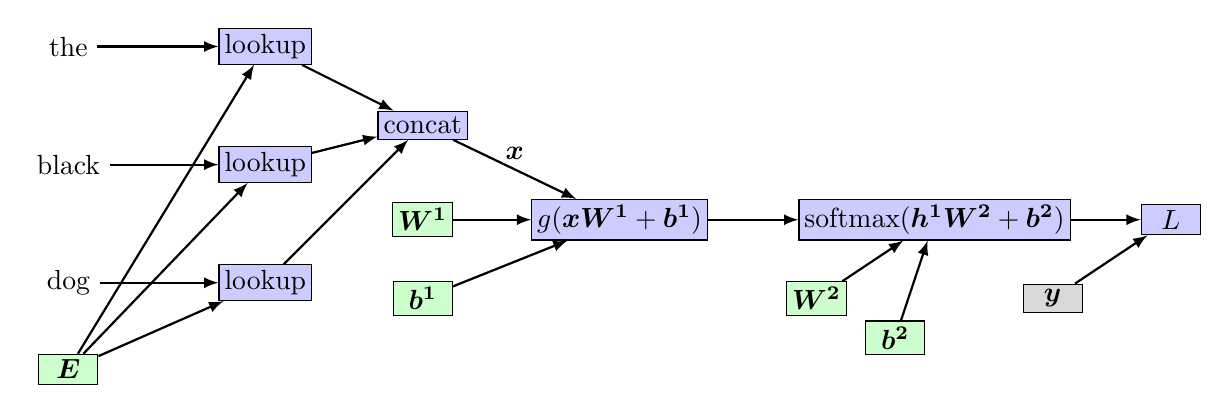
\begin{tikzpicture}	
			%\node (a1) [draw, circle, inner sep=0pt, minimum width=0.75cm, fill=green!20] {$a_1$};
			
			\node (the) {the};
			\node (black) [below of=the, yshift=-0.5cm]{black};
			\node (dog) [below of=black, yshift=-0.5cm]{dog};
			\node (e) [param, below of=dog, yshift=-0.1cm] {$\bm{E}$};
			
			\node (lookup1) [neuron, right of=the, xshift=1.5cm] {lookup};
			\node (lookup2) [neuron, below of=lookup1, yshift=-0.5cm] {lookup};
			\node (lookup3) [neuron, below of=lookup2, yshift=-0.5cm] {lookup};			
			\node (concat) [neuron, right of=lookup1, xshift=1cm, yshift=-1cm] {concat};
			
			
			%			\node (x) [constant, right of=concat, xshift=1cm] {$\bm{x}$};
			\node (w) [param, below of=concat, yshift=-0.2cm] {$\bm{W^1}$};
			\node (b) [param, below of=w] {$\bm{b^1}$};
			
			\node (f1) [neuron, right of=w, xshift=1.5cm] {$g(\bm{x} \bm{W^1} + \bm{b^1})$};
			
			\node (f2) [neuron, right of=f1, xshift=3cm] {$\softmax(\bm{h^1} \bm{W^2} + \bm{b^2})$};
			
			\node (w2) [param, below of=f2, xshift=-1.5cm, yshift=0cm] {$\bm{W^2}$};
			\node (b2) [param, below of=f2, xshift=-0.5cm, yshift=-0.5cm] {$\bm{b^2}$};
			
			\node (l) [neuron, right of=f2, xshift=2cm] {$L$};
			\node (y) [constant, below of=f2, xshift=1.5cm] {$\bm{y}$};
			
			\begin{scope}[thick, black, ->, >=latex]
				\draw (the) -- (lookup1);
				\draw (black) -- (lookup2);
				\draw (dog) -- (lookup3);
				\draw (e) -- (lookup1);
				\draw (e) -- (lookup2);
				\draw (e) -- (lookup3);
				
				\draw (lookup1) -- (concat);
				\draw (lookup2) -- (concat);
				\draw (lookup3) -- (concat);								
				
				\draw (concat) -- (f1) node [midway, above] {$\bm{x}$};
				\draw (w) -- (f1);
				\draw (b) -- (f1);
				\draw (f1) -- (f2);
				\draw (f2) -- (l);
				\draw (w2) -- (f2);
				\draw (b2) -- (f2);
				\draw (y) -- (l);
			\end{scope}	
		\end{tikzpicture}
	\end{figure}	
	
	Each word $\in \mathbb{R}^{\abs{V}}$ (one hot), 
	$\bm{E} \in \mathbb{R}^{\abs{V} \times 50}$, each lookup output $\in \mathbb{R}^{50}$, concat output $\bm{x} \in \mathbb{R}^{150}$
	
	
\end{frame}


\begin{frame}{Neural LMs}
	
	Let's build a neural network
	\begin{itemize}
		\item Input: a $k$-gram of words $w_{1:k}$
		\item Desired output: a probability distribution over the vocabulary $V$ for the next word $w_{k+1}$
	\end{itemize}
	
	Each input word $w_k$ is associated with an embedding vector $v(w) \in \mathbb{R}^{d_w}$ ($d_w$ --- word embedding dimensionality)
	
	Input vector $\bm{x}$ is a concatenation of $k$ words
	$$
	\bm{x} = \left[ v(w_1); v(w_2); \ldots; v(w_k) \right]
	$$
	
\end{frame}

\begin{frame}{Neural LMs}
	
	MLP with one (or more) hidden layers
	
	$$
	\begin{aligned}
		v(w) &= \bm{E}_{w,:} \\
		\bm{x} &= \left[ v(w_1); v(w_2); \ldots; v(w_k) \right] \\
		\bm{h} &= g(\bm{x} \bm{W^1} + \bm{b^1}) \\
		\hat{\bm{y}} = \Pr(W_i | w_{1:k}) &= \softmax (\bm{h} \bm{W^2} + \bm{b^2})
	\end{aligned}
	$$
	
	Output dimension: $\hat{\bm{y}} \in \mathbb{R}^{\abs{V}}$
	
\end{frame}

\begin{frame}{Training neural LMs}
	
	Where to get training examples?
	
	Training examples are simply word $k$-grams from an unlabeled corpus
	\begin{itemize}
		\item Identities of the first $k - 1$ words are used as features
		\item The last word is used as the target label for the classification
	\end{itemize}
	
	The model is trained using cross-entropy loss
\end{frame}

\begin{frame}{Some advantages and limitations of neural LMs}
	
	$\approx$ linear increase in parameters with $k + 1$ (better than `classical' LMs) but
	\begin{itemize}
		\item The size of the output vocabulary affects the computation time
		\item The softmax at the output layer requires an expensive matrix-vector multiplication with the matrix $\bm{W^2} \in \mathbb{R}^{d_{\text{hid} \times \abs{V}}}$, followed by $\abs{V}$ exponentiations
	\end{itemize}
	
	Solutions: Hierarchical softmax, noise-contrastive estimation
	
\end{frame}

\begin{frame}{Generating text with language models}
	
	We can generate (``sample") random sentences from the model according to their probability
	
	\begin{enumerate}
		\item Predict a probability distribution over the vocabulary conditioned on the start symbol <s>
		\item Draw a random word (the first word) according to the predicted distribution
		\item Predict a probability distribution over the vocabulary conditioned on the start symbol and the first word
		\item Draw a random word (the second word) according to the predicted distribution
		\item Repeat until generated \emph{end-of-sentence} symbol </s> (or <EOS>)
	\end{enumerate}
	
	
\end{frame}

\begin{frame}{Sampling words --- alternatives}
	
	Sampling (generating) the most probable word at each step might not be optimal globally
	
	\begin{itemize}
		\item Beam search --- generate top $k$ candidates at each step
	\end{itemize}
	
\end{frame}


\begin{frame}{Learned word representations as a by-product}
	\vspace{-1em}
	%	$$	f(\bm{x}) = g \left(	\bm{x} \bm{W^1} + \bm{b^1}	\right)	\bm{W^2} + \bm{b^2}	$$
	\begin{figure}
	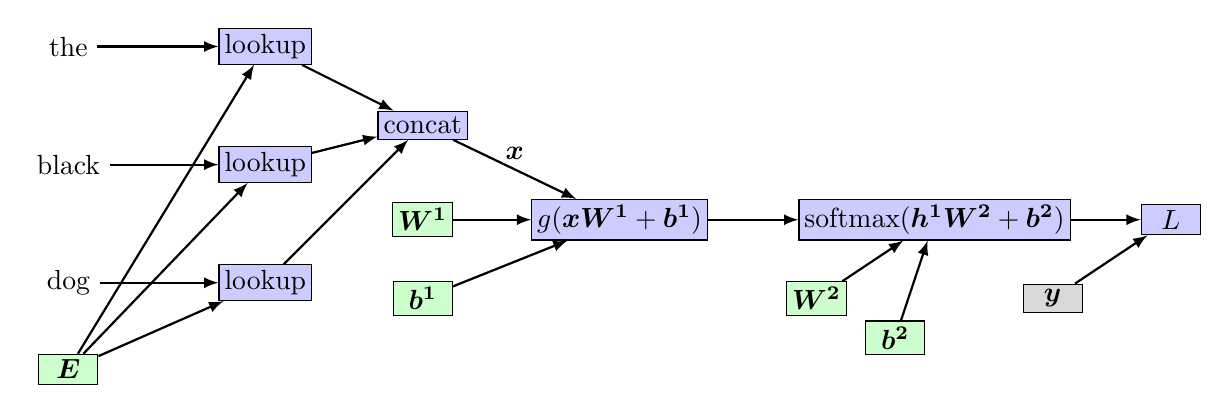
\begin{tikzpicture}	
		%\node (a1) [draw, circle, inner sep=0pt, minimum width=0.75cm, fill=green!20] {$a_1$};
		
		\node (the) {the};
		\node (black) [below of=the, yshift=-0.5cm]{black};
		\node (dog) [below of=black, yshift=-0.5cm]{dog};
		\node (e) [param, below of=dog, yshift=-0.1cm] {$\bm{E}$};
		
		\node (lookup1) [neuron, right of=the, xshift=1.5cm] {lookup};
		\node (lookup2) [neuron, below of=lookup1, yshift=-0.5cm] {lookup};
		\node (lookup3) [neuron, below of=lookup2, yshift=-0.5cm] {lookup};			
		\node (concat) [neuron, right of=lookup1, xshift=1cm, yshift=-1cm] {concat};
		
		
		%			\node (x) [constant, right of=concat, xshift=1cm] {$\bm{x}$};
		\node (w) [param, below of=concat, yshift=-0.2cm] {$\bm{W^1}$};
		\node (b) [param, below of=w] {$\bm{b^1}$};
		
		\node (f1) [neuron, right of=w, xshift=1.5cm] {$g(\bm{x} \bm{W^1} + \bm{b^1})$};
		
		\node (f2) [neuron, right of=f1, xshift=3cm] {$\softmax(\bm{h^1} \bm{W^2} + \bm{b^2})$};
		
		\node (w2) [param, below of=f2, xshift=-1.5cm, yshift=0cm] {$\bm{W^2}$};
		\node (b2) [param, below of=f2, xshift=-0.5cm, yshift=-0.5cm] {$\bm{b^2}$};
		
		\node (l) [neuron, right of=f2, xshift=2cm] {$L$};
		\node (y) [constant, below of=f2, xshift=1.5cm] {$\bm{y}$};
		
		\begin{scope}[thick, black, ->, >=latex]
			\draw (the) -- (lookup1);
			\draw (black) -- (lookup2);
			\draw (dog) -- (lookup3);
			\draw (e) -- (lookup1);
			\draw (e) -- (lookup2);
			\draw (e) -- (lookup3);
			
			\draw (lookup1) -- (concat);
			\draw (lookup2) -- (concat);
			\draw (lookup3) -- (concat);								
			
			\draw (concat) -- (f1) node [midway, above] {$\bm{x}$};
			\draw (w) -- (f1);
			\draw (b) -- (f1);
			\draw (f1) -- (f2);
			\draw (f2) -- (l);
			\draw (w2) -- (f2);
			\draw (b2) -- (f2);
			\draw (y) -- (l);
		\end{scope}	
	\end{tikzpicture}
\end{figure}	
	
	Each row of $\bm{E}$ learns a word representation
	
	Each column of $\bm{W^2}$ learns a word representation
	
\end{frame}

\section{Word embeddings}

\begin{frame}{Word embeddings as pre-trained word representation}
	
	Option A: We can initialize the embeddings matrix $\bm{E}$ randomly and learn during our supervised task
	
	Option B: Use pre-trained word embeddings from task for which we have a lot of data
	
	\begin{itemize}
		\item Use self-supervised learning (create labeled data `for free' using the next word prediction objective)
		\item Learned word embedding matrix plugged into our supervised task
	\end{itemize}
	
	Desired word embeddings properties: `Similar' words have similar embeddings vectors
\end{frame}


\section*{Recap}






\begin{frame}{Take aways}
	
	\begin{itemize}
		\item Language modeling is an essential part of contemporary NLP
		\item Self-supervised models, unlabeled data, next word prediction
		\item Neural language models learn embedding of words
	\end{itemize}
	
\end{frame}





\begin{frame}{License and credits}

	\begin{columns}
		\begin{column}{0.7\textwidth}
			Licensed under Creative Commons Attribution-ShareAlike 4.0 International (CC BY-SA 4.0)
		\end{column}
		\begin{column}{0.2\textwidth}
			
\includegraphics[width=0.9\linewidth]{img/cc-by-sa-icon.pdf}
		\end{column}
	\end{columns}
	
	\bigskip
	
	Credits
	
	\begin{scriptsize}
		
		Ivan Habernal
		
		Content from ACL Anthology papers licensed under CC-BY \url{https://www.aclweb.org/anthology}
		
	\end{scriptsize}
	
\end{frame}



\end{document}

